\documentclass[11pt]{article} % Font size (can be 10pt, 11pt or 12pt) and paper size (remove a4paper for US letter paper)

\usepackage{amsmath,amssymb,amsthm,gensymb}

\usepackage{geometry}
\usepackage{wrapfig}
\usepackage{hyperref}
\usepackage{makecell}

\hypersetup{
    colorlinks=true,
    linkcolor=black,
    filecolor=magenta,      
    urlcolor=blue,
}
\usepackage[protrusion=true,expansion=true]{microtype} % Better typography
\usepackage{hyperref}
\usepackage{graphicx} % Required for including pictures
\usepackage{wrapfig} % Allows in-line images
\linespread{1.12}
\usepackage{mathtools}
\usepackage[font=footnotesize,labelfont=bf]{caption}
\usepackage[T1]{fontenc} % Required for accented characters

\makeatletter

\newcommand{\bra}[1]{\left\langle #1 \right|}
\newcommand{\ket}[1]{\left|#1\right\rangle}
\newcommand{\braket}[2]{\left\langle#1 |  #2\right\rangle}
\makeatother

%\addbibresource{bibliography.bib}


\author{Amir Karamlou\footnote{Notes LaTeXed by Megan Yamoah for 6.s089 IAP 2019 and Grecia Castelazo for 6.s089 IAP 2020.}, Francisca Vasconcelos \\\href{mailto:karamlou@mit.edu} {karamlou@mit.edu}, \href{mailto:francisc@mit.edu}{francisc@mit.edu}}
\title{Introduction to Quantum Computing\\Lecture 4: Applications of Quantum Circuits}
\date{Massachusetts Institute of Technology\\6.s089 IAP 2020}

\begin{document}
\maketitle
\newpage
\tableofcontents
\newpage

\section{Superdense Coding}\label{superdense}
Let's say Alice (A) and Bob (B) share an entangled pair:
\begin{align}
    \ket{\beta_{00}}=\frac{\ket{00}+\ket{11}}{\sqrt{2}}.
    \label{beta00}
\end{align}
We can created this entagled state by taking starting their qubits in the $\ket{0}$ state, applying a Hadamard $H$ on Alice's qubit, and finally applying a CNOT with Alice's qubit has the control.

Now, we ask: how does Alice transmit certain sets of information? Well, we must encode our possible bits:
\begin{table}[!htbp]
    \centering
    \begin{tabular}{c|c c}
        message & transformation & result\\\hline
        00 & $\mathbb{I}_A\otimes\mathbb{I}_B$ & $\frac{\ket{00}+\ket{11}}{\sqrt{2}}=\ket{\beta_{00}}$\\
        00 & $X_A\otimes\mathbb{I}_B$ & $\frac{\ket{10}+\ket{01}}{\sqrt{2}}=\ket{\beta_{01}}$\\
        10 & $Z_A\otimes\mathbb{I}_B$ & $\frac{\ket{00}-\ket{11}}{\sqrt{2}}=\ket{\beta_{10}}$\\
        11 & $X_A,Z_A\otimes\mathbb{I}_B$ & $\frac{\ket{10}-\ket{01}}{\sqrt{2}}=\ket{\beta_{11}}$\\
    \end{tabular}
\end{table}
In short, Alice performs certain operations on her qubit to encode a two-bit value before sending her qubit to Bob. Bob then makes a ``Bell measurement". A ``Bell measurement" simply unentangles an entagled state. Namely, he applies a CNOT with Alice's qubit as the control and then applies a Hadamard on Alice's qubit before measuring. Working this out, we will find that Bob will simply measure Alice's original two-bit states.

\newpage

\section{Quantum Teleportation}
While this subject is rather over-hyped, it is indeed true that quantum mechanics can lead to a certain kind of state teleportation. First, let's again begin with our friends Alice and Bob. Say they share the entangled state from Eq. \ref{beta00}, $\ket{\beta_{00}}$. Now, Alice wants to teleport a separate state $\ket{\psi}=\alpha\ket{0}+\beta\ket{1}$. The full system state is then:
\begin{align}
    \ket{\psi}\otimes\ket{\beta_{00}} =&\left(\alpha\ket{0}+\beta\ket{1}\right)\otimes\frac{\ket{00}+\ket{11}}{\sqrt{2}}\\
    =&\frac{1}{2\sqrt{2}}(\ket{00}+\ket{11})_A\otimes\left(\alpha\ket{0}+\beta\ket{1}\right)_B\nonumber\\
    &+\frac{1}{2\sqrt{2}}(\ket{01}+\ket{10})_A\otimes\left(\alpha\ket{0}+\beta\ket{1}\right)_B\nonumber\\
    &+\frac{1}{2\sqrt{2}}(\ket{00}-\ket{11})_A\otimes\left(\alpha\ket{0}-\beta\ket{1}\right)_B\nonumber\\
    &+\frac{1}{2\sqrt{2}}(\ket{01}-\ket{10})_A\otimes\left(\alpha\ket{0}-\beta\ket{1}\right)_B.
\end{align}

Now, Alice applies a CNOT with her state $\ket{\psi}$ as the control and her qubit of the entangled pair as the target and then performs a Hadamard on the state $\ket{\psi}$. This is the Bell measurement disucussed in Section \ref{superdense}. This means that Alice's qubit is now encoded into a two-bit value which can then be used to perform operations on Bob's half of the entagled pair. After the CNOT, we find:
\begin{align}
    U_{CNOT}\ket{\psi}\otimes\ket{\beta_{00}} 
    =&\frac{1}{2\sqrt{2}}(\ket{00}+\ket{10})_A\otimes\left(\alpha\ket{0}+\beta\ket{1}\right)_B\nonumber\\
    &+\frac{1}{2\sqrt{2}}(\ket{01}+\ket{11})_A\otimes\left(\alpha\ket{1}+\beta\ket{0}\right)_B\nonumber\\
    &+\frac{1}{2\sqrt{2}}(\ket{00}-\ket{10})_A\otimes\left(\alpha\ket{0}-\beta\ket{1}\right)_B\nonumber\\
    &+\frac{1}{2\sqrt{2}}(\ket{01}-\ket{11})_A\otimes\left(\alpha\ket{1}-\beta\ket{0}\right)_B
\end{align}
Now performing the Hadamard and measuring Alice's two qubits (her $\ket{\psi}$ and entangled qubit), we know which state Bob holds based on the measurement of Alice's qubits. Namely, she measures 00, 01, 10, 11 based on the Bell measurement we discussed above. This measurement then collapses Bob's state to $\alpha\ket{0}+\beta\ket{1}$, $\alpha\ket{1}+\beta\ket{0}$, $\alpha\ket{0}-\beta\ket{1}$, or $\alpha\ket{1}-\beta\ket{0}$, respectively. As such, we can use Alice's measurement to perform transformations on Bob's qubit such that Bob ends with the original state $\ket{\psi}=\alpha\ket{0}+\beta\ket{1}$. Specifically, we would apply an X operation if Alice's first bit is 1 and a Z operation if Alice's second bit is 1.

\section{Deutsch-Josza Algorithm}
The Deutsch-Josza algorithm, named after David Deutsch and Richard Jozsa, is a simple demonstration of quantum speed-up. It allows us to determine whether a binary function $f$, ($f: \{0,1\} \rightarrow \{0,1\}$) is fixed (i.e. $f(x)=0$ or $f(x)=1$ for all $x$) or variable (i.e., $f(x)=0$ and $f(x)=1$ for exactly half of their inputs).
\begin{equation}
     \label{eq:f1}
     f(x) = \left\{
	       \begin{array}{ll}
		 0 \mathrm{\ or\ } 1      & \mathrm{for\ all\ } x \mathrm{\ if\ } f \mathrm{\ is\ fixed\ }\\
		 0 \mathrm{\ or\ } 1      & \mathrm{for\ half\ the\ inputs\ } \mathrm{if\ } f \mathrm{\ is\ variable}\\
	       \end{array}
	     \right.
   \end{equation}
%\begin{equation}
%     \label{eq:f2}
%     f(x) = \left\{
%	       \begin{array}{ll}
%		 c      & \mathrm{\ if\ } f \mathrm{\ is\ fixed\ }\\
%		 x      & \mathrm{if\ } f \mathrm{\ is\ variable}\\
%	       \end{array}
%	     \right.
%   \end{equation}
From a classical point of view, it necessarily takes two calls to determine whether the function $f$ in the black box is fixed or variable. However, using quantum information processing this can be accomplished using one call.\\
Define a unitary operation $U_f$ such that $\ket{x} \otimes \ket{y} \rightarrow \ket{x} \otimes \ket{y \oplus f(x)}$.

\begin{figure}[h!]
    \centering
    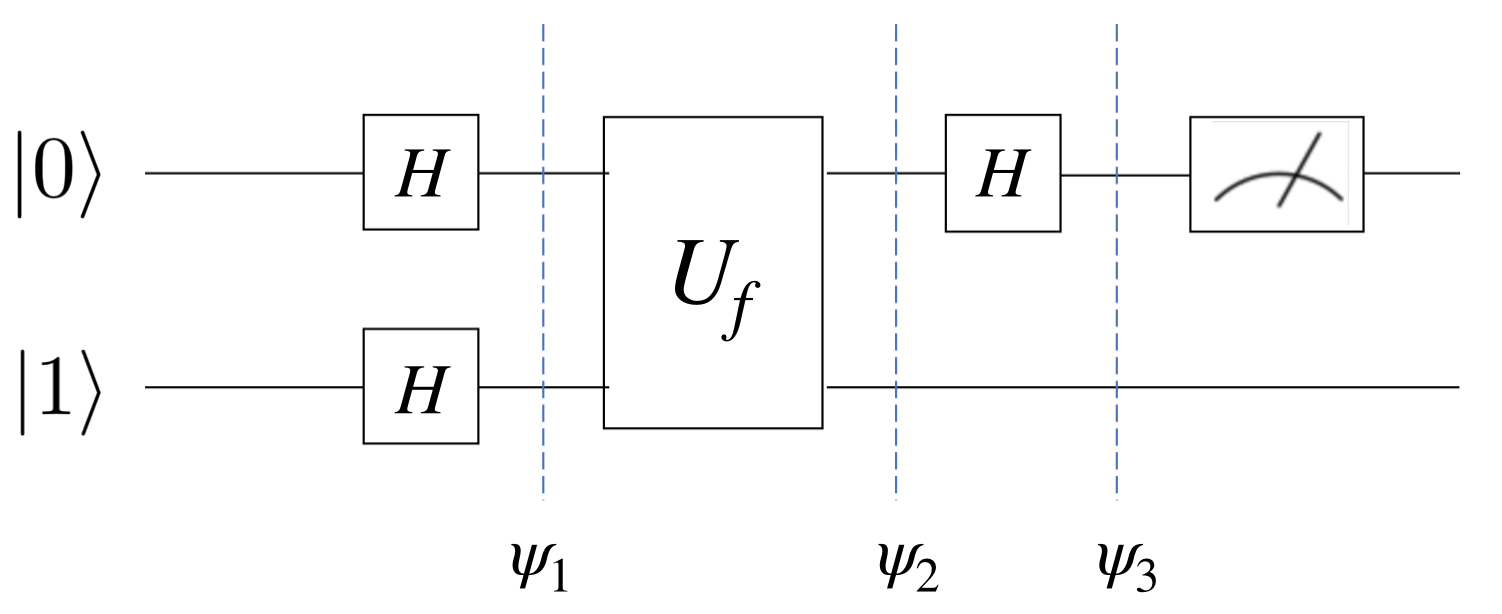
\includegraphics[width=.6\textwidth]{Lecture4Figs/DeutschJozsa-diag.png}
    \caption{Deutsch-Jozsa algorithm circuit for two qubits for an input $\ket{\psi_0}=\ket{x}\ket{y} \rightarrow \ket{0}\ket{1}$. Measurement on the first output yields $0$ when $f$ is fixed and $1$ when $f$ is variable.}
    \label{fig:Deutsch-Jozsa}
\end{figure}
In the case of Fig.\ref{fig:Deutsch-Jozsa}, $\ket{\psi_1}$ can be written as
\begin{align}
    \ket{\psi_1}: \ket{+}\otimes\ket{-} 
    =&\Big(\frac{\ket{0}+\ket{1}}{\sqrt{2}}\Big)\otimes \Big(\frac{\ket{0}-\ket{1}}{\sqrt{2}}\Big)\\
    =&\frac{1}{2}(\ket{0}\ket{0}-\ket{0}\ket{1}+\ket{1}\ket{0}-\ket{1}\ket{1}).
\end{align}
After applying the $U_f$ operator,
\begin{align}
    \ket{\psi_2}: \
    &\frac{1}{2}(\ket{0}\ket{f(0)}-\ket{0}\ket{1\oplus f(0)}+\ket{1}\ket{f(1)}-\ket{1}\ket{1\oplus f(1)})\\
    &=\frac{(-1)^{f(0)}}{\sqrt{2}}\ket{0}\Big(\frac{\ket{0}-\ket{1}}{\sqrt{2}} \Big)+\frac{(-1)^{f(1)}}{\sqrt{2}}\ket{1}\Big(\frac{\ket{0}-\ket{1}}{\sqrt{2}} \Big).
\end{align}
If $f$ is fixed: 
\begin{align}
    &\ket{\psi_2} \rightarrow \Big(\frac{\ket{0}+\ket{1}}{\sqrt{2}}\Big)\otimes\Big(\frac{\ket{0}-\ket{1}}{\sqrt{2}}\Big) \\
    & \ket{\psi_3}: H\otimes I\ket{\psi_2}\\
    =& \ket{0}\otimes\Big(\frac{\ket{0}-\ket{1}}{\sqrt{2}} \Big)=\ket{0}\otimes\ket{-}.
\end{align}
If $f$ is variable: 
\begin{align}
    &\ket{\psi_2} \rightarrow \pm \ \Big(\frac{\ket{0}-\ket{1}}{\sqrt{2}}\Big)\otimes\Big(\frac{\ket{0}-\ket{1}}{\sqrt{2}}\Big) \\
    & \ket{\psi_3}: H\otimes I\ket{\psi_2}\\
    =& \ket{1}\otimes\Big(\frac{\ket{0}+\ket{1}}{\sqrt{2}} \Big)=\ket{1}\otimes\ket{+}.
\end{align}
We conclude that the output on the first qubit yields a $0$ when $f$ is fixed and $1$ when $f$, therefore determining whether $f$ is constant or balanced using one single query, as desired.
\\We refer to the description in the book \textit{Introduction to Quantum Computing} by Phillip Kaye and Raymond Laflamme (posted on course page).


\newpage
\section{Quantum Cryptography}

\textit{Quantum cryptography} is the field of study dedicated to exploiting quantum mechanics to perform cryptographic tasks. This should not be confused with \textit{post-quantum cryptography}, which is the field devoted to studying cryptography algorithms which are robust to attack by quantum computers. We will explore post-quantum cryptography a little when we discuss Shor's algorithm, but for now we focus on the first ever quantum cryptography protocol: BB84.

\subsection{Classical Key Distribution}
Before diving into quantum key distribution, we must first understand its classical analog and why it is important/useful. Although classical cryptography is a rich field, for the purposes of this class we will consider two main types of key distribution: symmetric key cryptography and public key cryptography. Public key cryptography will become important when we discuss RSA later in the course. For now, we focus on \textit{symmetric key cryptography}.

\begin{figure}[h!]
    \centering
    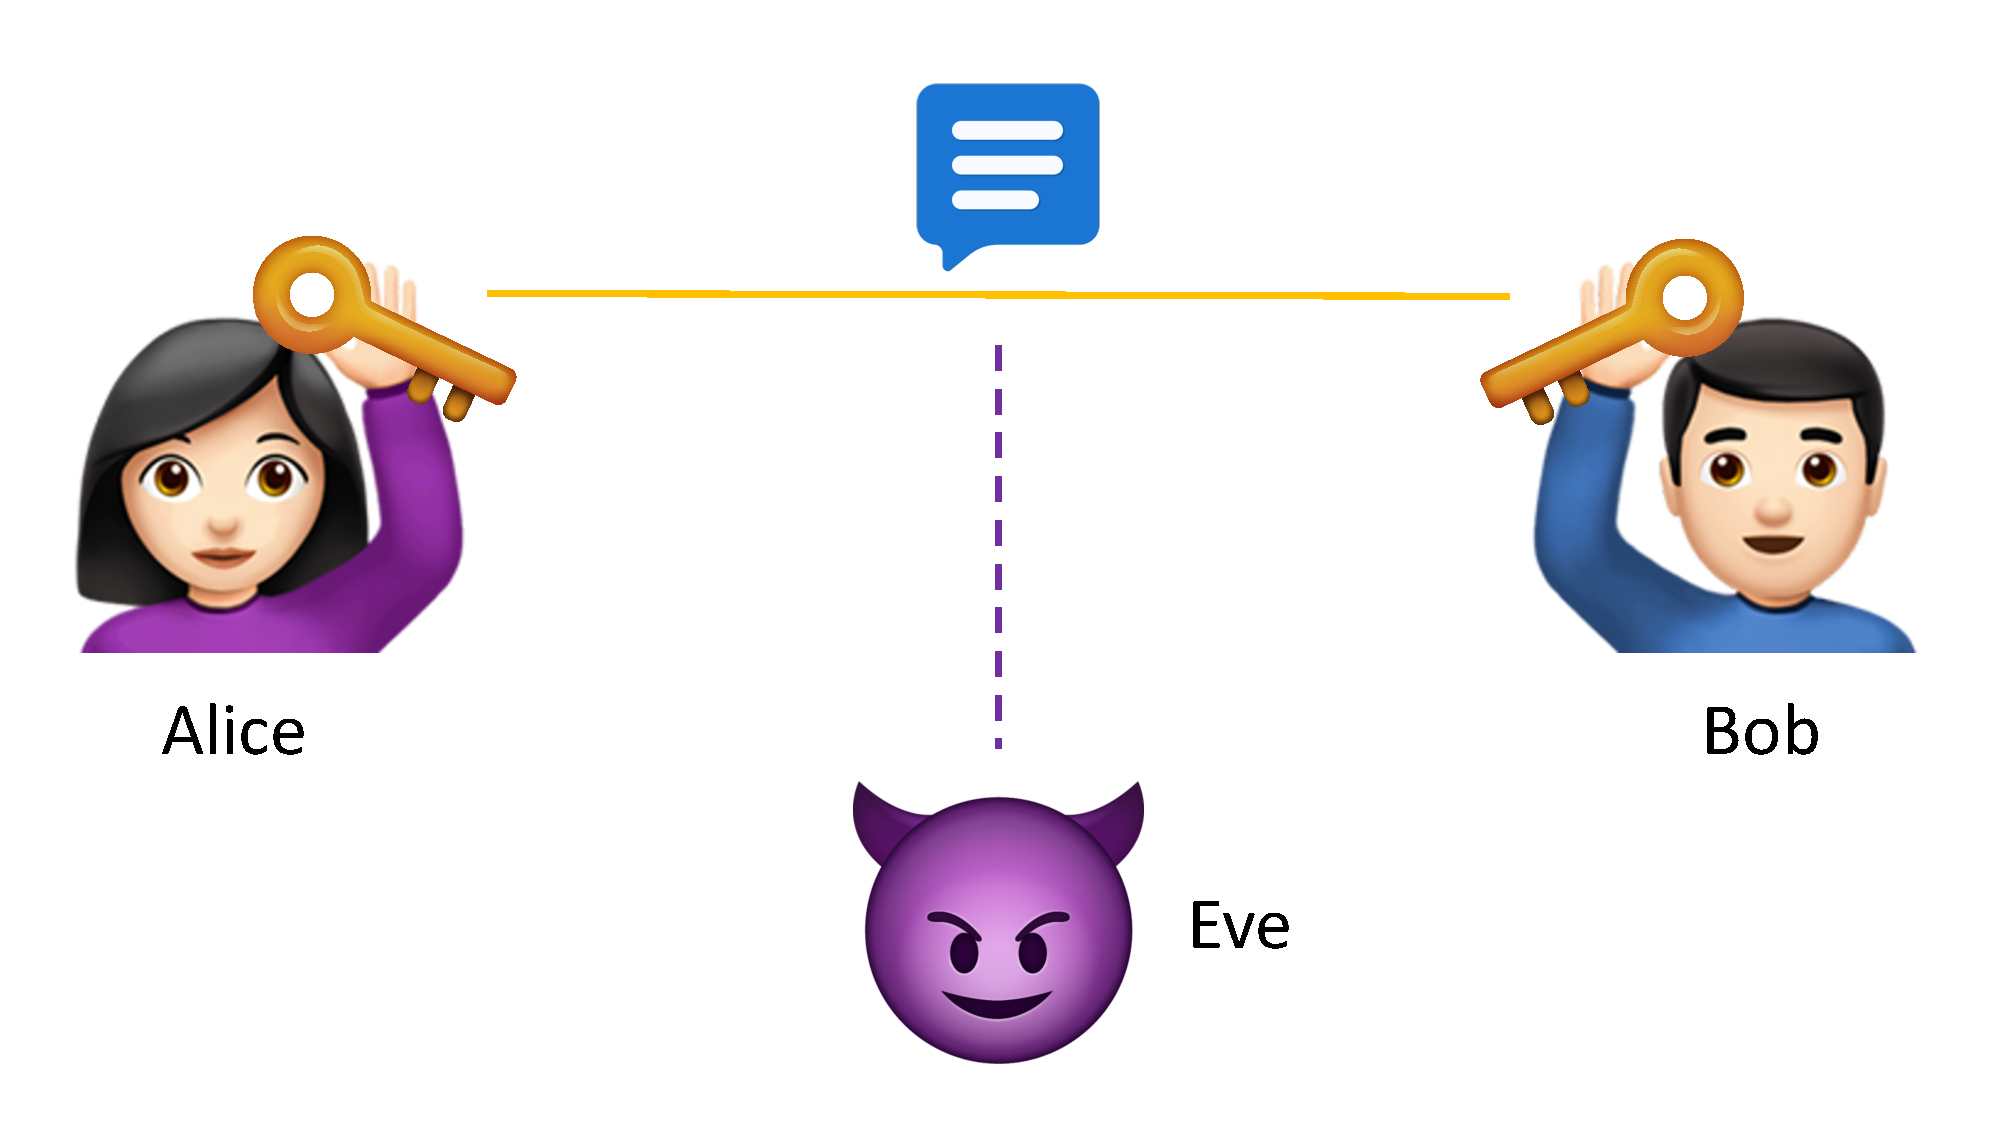
\includegraphics[width=.7\textwidth]{Lecture4Figs/SymmetricKeyDist.pdf}
    \caption{Symmetric key cryptography, with messaging parties Alice and Bob, being eavesdropped by Eve.}
    \label{fig:QKD}
\end{figure}

In symmetric key cryptography, there are two parties, which we refer to as Alice and Bob, who are trying to exchange a private message. However, they are aware that an eavesdropper, Eve, is trying to listen in on their conversation for malicious purposes. Thus, in order to protect their message, they decide to use a shared private \textit{key}. 

A key is simply a number (a string of 0's and 1's) and the larger the key, the better (since it is harder to guess). In the case of symmetric key cryptography, since both Alice and Bob have access to the same key, this key is used to both \textit{encrypt} and \textit{decrypt} the message. There are several codes that can use a key to encrypt and decrypt a message, such as stream ciphers or block ciphers. 

In the classical setting, the main challenge with symmetric key cryptography is actually getting the same key to both Alice and Bob. If Alice generates the key, the only ways she can get it to Bob are via a face-to-face meeting, use of a trusted courier, or sending the key through a pre-existing encryption channel. The meeting and courier are usually impractical and always insecure, since the key can be intercepted. The use of a previously established communication channel depends on the security of a previous key exchange. Thus, Alice and Bob turn to quantum mechanics to distribute their key in a secure fashion (or at least to know if someone else is intercepting their messages).

\subsection{BB84 QKD Protocol}

BB84 gets its name from the fact that it was developed by Charles Bennett and Gilles Brassard in 1984. It is a \textit{quantum key distribution} protocol, which means that it uses quantum mechanics in order to distribute the symmetric key we previously discussed.

Imagine that Alice has generated a key and wants to share the key with Bob, in order to send a message. She has two communication channels with Bob. The first is a classical communication channel, for example a telephone. This channel can be public and we will see why shortly. The second is a quantum channel, such as an optical fiber cable to send polarized light. Ideally this channel would be secure, but Alice and Bob have suspicions that Eve has tapped the wire and is intercepting photons being transmitted to Bob. 

At this point, it should be noted that the BB84 protocol does not prevent Eve from intercepting the message. Instead, it allows Alice and Bob to statistically deduce \textit{if} Eve has tapped into the quantum communication channel. If so, they know that their quantum communication channel is not secure and that they should disregard the key. They will then need to find another quantum communication channel and try again.

\subsubsection{Overview}
Now, lets dive into the procedure for transmitting and analyzing the key. Begin with assumption that Alice and Bob have already established the length of the key ($n$) and the two possible bases to polarize/measure the light for their quantum communication channel:
\begin{enumerate}
    \item Horizontal-Vertical Polarization ($\pmb{+}$), with basis states: $|\uparrow\rangle$, $|\rightarrow\rangle$
    \item Diagonal Polarization ($\bigtimes$), with basis states: $|\nearrow\rangle$, $|\searrow\rangle$
\end{enumerate}
There are five key steps to the BB84 protocol:
\begin{enumerate}
    \item For each of the $n$ bits, Alice randomly selects a basis ($\pmb{+}$ or $\bigtimes$) to encode that bit.
    \item For each of the $n$ bits, Bob randomly selects a basis ($\pmb{+}$ or $\bigtimes$) to measure that bit.
    \item Alice creates the polarized bit states and sends them to Bob, who measures them (in the pre-determined bases). 
    \item After all $n$ bits are measured by Bob (in the quantum channel), Alice announces which basis she used to encode each bit (in the public channel) as well as a certain number of the bits originally sent.
    \item Analysis is performed to determine if the message was intercepted by Eve. If so, Alice and Bob should move to a new quantum communication channel and try again. If not, a key was transmitted and Alice can send her full message using the key for encryption. Bob can decode the message using the key.
\end{enumerate}

\subsubsection{Analysis (without Eve)}
For the purpose of simplifying our analysis, we will assume that the random basis selection technique used by Alice and Bob is flipping a coin for each bit. If heads, the bit is encoded/measured in the  $\bigtimes$ basis. If tails, the bit is encoded/measured in the  $\pmb{+}$ basis. Note that Alice and Bob are \textit{independently} flipping coins and have no knowledge of each other's bases until after Bob measures all the transmitted quantum states. For now, we also assume that there is no noise present in the quantum communication channel. 

\begin{table}[h!]
    \centering
    \begin{tabular}{c|cc|cc|c}
         Key Bit & Alice Basis & Transmitted State & Bob Basis & Measured State & Shared Key \\
         \hline
         0 & $\pmb{+}$ & $|\uparrow\rangle$ & $\pmb{+}$ & $|\uparrow\rangle$ & 0 \\
         \hline
         0 & $\pmb{+}$ & $|\uparrow\rangle$ & $\bigtimes$ & \makecell{$|\nearrow\rangle$ - 50\% \\ $|\searrow\rangle$ - 50\%} & - \\
         \hline
         0 & $\bigtimes$ & $|\nearrow\rangle$ & $\pmb{+}$ & \makecell{$|\uparrow\rangle$ - 50\% \\ $|\downarrow\rangle$ - 50\%} & - \\
         \hline
         0 & $\bigtimes$ & $|\nearrow\rangle$ & $\bigtimes$ & $|\nearrow\rangle$ & 0 \\
         \hline
         1 & $\pmb{+}$ & $|\rightarrow\rangle$ & $\pmb{+}$ & $|\rightarrow\rangle$ & 1 \\
         \hline
         1 & $\pmb{+}$ & $|\rightarrow\rangle$ & $\bigtimes$ & \makecell{$|\nearrow\rangle$ - 50\% \\ $|\searrow\rangle$ - 50\%} & - \\
         \hline
         1 & $\bigtimes$ & $|\searrow\rangle$ & $\pmb{+}$ & \makecell{$|\uparrow\rangle$ - 50\% \\ $|\downarrow\rangle$ - 50\%} & - \\
         \hline
         1 & $\bigtimes$ & $|\searrow\rangle$ & $\bigtimes$ & $|\searrow\rangle$ & 1 \\
    \end{tabular}
    \caption{BB84 state preparation and measurement (assuming no eavesdropper or noise).}
    \label{tab:qkd}
\end{table}

Now, let's see how the experiment would look if there was no eavesdropper. In Table~\ref{tab:qkd}, we summarize all the possible ways a bit transmission can occur. If Alice and Bob choose the same basis (which happens 50\% of the time), the transmitted and measured states are equivalent. However, if Alice and Bob choose different states, the measured state is only equivalent to the transmitted state 50\% of the time. Since Alice never explicitly tells Bob which state she sent (nor does Bob ever state which state he measures), they must disregard any bits for which they did not measure in the same basis. Thus, if there was no noise or eavesdropper on the line, Alice and Bob would end up on average with an agreed key of length $\frac{n}{2}$.



\subsubsection{Analysis (with Eve)}
Still assuming that there is no noise in the quantum channel, we now consider what happens when Eve is present. If Eve can tap into the quantum channel, she can intercept the photons Alice is transmitting to Bob. However, by the No-Cloning Theorem, she cannot actually make a copy of the photon state. Thus, Eve must measure the intercepted photon. 

Eve is sneaky and already knows about the form of the experiment, including the two different measurement bases being used. Thus, similarly to Bob, each time she must randomly select a basis to measure the photon in. She can then record what she sees, but must transmit the measured photon to Bob, so as not to arouse suspicions. Bob will then proceed to measure those photons, unaware that they have already been measured. 

Once Bob has declared that he has measured the final bit, Alice will communicate her measurement bases over the classical channel, which we know Eve has access to. Thus, Eve knows that whenever she selected the same basis as Alice (which happens 50\% of the time), she knows the transmitted bit. However, since the whole transmission is just of a key and not the actual message, Eve has not yet gained any useful information. Bob also takes notes of which bits he measured in the same basis and informs Alice.

Now, in order to determine whether Eve was listening in or not, a final piece of information must be transmitted over the classical line. Among all the bits for which Alice and Bob encoded/measured in the same basis, we would expect that Alice only guessed the correct basis 50\% of the time. Thus, even though Bob should measure the same bit that Alice transmitted (again assuming no noise), 50\% of the time Alice changed the measurement basis, meaning 25\% of the time we would expect Bob to measure a different bit from the transmitted one. Thus, Alice can reveal a certain number of her transmitted bits (among those for which the bases matched), so as to determine whether or not Eve was on the line. In the case of no noise, if any of Bob's measurements do not match Alice's transmitted bit then there must be an eavesdropped. However, Alice cannot announce all the bits over the classical line, because it is an insecure channel and someone could just be listening in on that (without accessing the quantum channel).

The exact number of bits that Alice should transmit as well as estimates of the number of experiment repetitions required to transmit a key of certain length can be calculated using information reconciliation and privacy amplification techniques. However, these lie outside of the scope of this course. 


\end{document}